% Options for packages loaded elsewhere
\PassOptionsToPackage{unicode}{hyperref}
\PassOptionsToPackage{hyphens}{url}
%
\documentclass[
]{book}
\usepackage{amsmath,amssymb}
\usepackage{lmodern}
\usepackage{iftex}
\ifPDFTeX
  \usepackage[T1]{fontenc}
  \usepackage[utf8]{inputenc}
  \usepackage{textcomp} % provide euro and other symbols
\else % if luatex or xetex
  \usepackage{unicode-math}
  \defaultfontfeatures{Scale=MatchLowercase}
  \defaultfontfeatures[\rmfamily]{Ligatures=TeX,Scale=1}
\fi
% Use upquote if available, for straight quotes in verbatim environments
\IfFileExists{upquote.sty}{\usepackage{upquote}}{}
\IfFileExists{microtype.sty}{% use microtype if available
  \usepackage[]{microtype}
  \UseMicrotypeSet[protrusion]{basicmath} % disable protrusion for tt fonts
}{}
\makeatletter
\@ifundefined{KOMAClassName}{% if non-KOMA class
  \IfFileExists{parskip.sty}{%
    \usepackage{parskip}
  }{% else
    \setlength{\parindent}{0pt}
    \setlength{\parskip}{6pt plus 2pt minus 1pt}}
}{% if KOMA class
  \KOMAoptions{parskip=half}}
\makeatother
\usepackage{xcolor}
\usepackage{color}
\usepackage{fancyvrb}
\newcommand{\VerbBar}{|}
\newcommand{\VERB}{\Verb[commandchars=\\\{\}]}
\DefineVerbatimEnvironment{Highlighting}{Verbatim}{commandchars=\\\{\}}
% Add ',fontsize=\small' for more characters per line
\usepackage{framed}
\definecolor{shadecolor}{RGB}{248,248,248}
\newenvironment{Shaded}{\begin{snugshade}}{\end{snugshade}}
\newcommand{\AlertTok}[1]{\textcolor[rgb]{0.94,0.16,0.16}{#1}}
\newcommand{\AnnotationTok}[1]{\textcolor[rgb]{0.56,0.35,0.01}{\textbf{\textit{#1}}}}
\newcommand{\AttributeTok}[1]{\textcolor[rgb]{0.77,0.63,0.00}{#1}}
\newcommand{\BaseNTok}[1]{\textcolor[rgb]{0.00,0.00,0.81}{#1}}
\newcommand{\BuiltInTok}[1]{#1}
\newcommand{\CharTok}[1]{\textcolor[rgb]{0.31,0.60,0.02}{#1}}
\newcommand{\CommentTok}[1]{\textcolor[rgb]{0.56,0.35,0.01}{\textit{#1}}}
\newcommand{\CommentVarTok}[1]{\textcolor[rgb]{0.56,0.35,0.01}{\textbf{\textit{#1}}}}
\newcommand{\ConstantTok}[1]{\textcolor[rgb]{0.00,0.00,0.00}{#1}}
\newcommand{\ControlFlowTok}[1]{\textcolor[rgb]{0.13,0.29,0.53}{\textbf{#1}}}
\newcommand{\DataTypeTok}[1]{\textcolor[rgb]{0.13,0.29,0.53}{#1}}
\newcommand{\DecValTok}[1]{\textcolor[rgb]{0.00,0.00,0.81}{#1}}
\newcommand{\DocumentationTok}[1]{\textcolor[rgb]{0.56,0.35,0.01}{\textbf{\textit{#1}}}}
\newcommand{\ErrorTok}[1]{\textcolor[rgb]{0.64,0.00,0.00}{\textbf{#1}}}
\newcommand{\ExtensionTok}[1]{#1}
\newcommand{\FloatTok}[1]{\textcolor[rgb]{0.00,0.00,0.81}{#1}}
\newcommand{\FunctionTok}[1]{\textcolor[rgb]{0.00,0.00,0.00}{#1}}
\newcommand{\ImportTok}[1]{#1}
\newcommand{\InformationTok}[1]{\textcolor[rgb]{0.56,0.35,0.01}{\textbf{\textit{#1}}}}
\newcommand{\KeywordTok}[1]{\textcolor[rgb]{0.13,0.29,0.53}{\textbf{#1}}}
\newcommand{\NormalTok}[1]{#1}
\newcommand{\OperatorTok}[1]{\textcolor[rgb]{0.81,0.36,0.00}{\textbf{#1}}}
\newcommand{\OtherTok}[1]{\textcolor[rgb]{0.56,0.35,0.01}{#1}}
\newcommand{\PreprocessorTok}[1]{\textcolor[rgb]{0.56,0.35,0.01}{\textit{#1}}}
\newcommand{\RegionMarkerTok}[1]{#1}
\newcommand{\SpecialCharTok}[1]{\textcolor[rgb]{0.00,0.00,0.00}{#1}}
\newcommand{\SpecialStringTok}[1]{\textcolor[rgb]{0.31,0.60,0.02}{#1}}
\newcommand{\StringTok}[1]{\textcolor[rgb]{0.31,0.60,0.02}{#1}}
\newcommand{\VariableTok}[1]{\textcolor[rgb]{0.00,0.00,0.00}{#1}}
\newcommand{\VerbatimStringTok}[1]{\textcolor[rgb]{0.31,0.60,0.02}{#1}}
\newcommand{\WarningTok}[1]{\textcolor[rgb]{0.56,0.35,0.01}{\textbf{\textit{#1}}}}
\usepackage{longtable,booktabs,array}
\usepackage{calc} % for calculating minipage widths
% Correct order of tables after \paragraph or \subparagraph
\usepackage{etoolbox}
\makeatletter
\patchcmd\longtable{\par}{\if@noskipsec\mbox{}\fi\par}{}{}
\makeatother
% Allow footnotes in longtable head/foot
\IfFileExists{footnotehyper.sty}{\usepackage{footnotehyper}}{\usepackage{footnote}}
\makesavenoteenv{longtable}
\usepackage{graphicx}
\makeatletter
\def\maxwidth{\ifdim\Gin@nat@width>\linewidth\linewidth\else\Gin@nat@width\fi}
\def\maxheight{\ifdim\Gin@nat@height>\textheight\textheight\else\Gin@nat@height\fi}
\makeatother
% Scale images if necessary, so that they will not overflow the page
% margins by default, and it is still possible to overwrite the defaults
% using explicit options in \includegraphics[width, height, ...]{}
\setkeys{Gin}{width=\maxwidth,height=\maxheight,keepaspectratio}
% Set default figure placement to htbp
\makeatletter
\def\fps@figure{htbp}
\makeatother
\setlength{\emergencystretch}{3em} % prevent overfull lines
\providecommand{\tightlist}{%
  \setlength{\itemsep}{0pt}\setlength{\parskip}{0pt}}
\setcounter{secnumdepth}{5}
\usepackage{booktabs}
\ifLuaTeX
  \usepackage{selnolig}  % disable illegal ligatures
\fi
\usepackage[]{natbib}
\bibliographystyle{plainnat}
\IfFileExists{bookmark.sty}{\usepackage{bookmark}}{\usepackage{hyperref}}
\IfFileExists{xurl.sty}{\usepackage{xurl}}{} % add URL line breaks if available
\urlstyle{same} % disable monospaced font for URLs
\hypersetup{
  pdftitle={pdmphmc - numerical generalized randomized HMC processes for R},
  pdfauthor={Tore Selland Kleppe},
  hidelinks,
  pdfcreator={LaTeX via pandoc}}

\title{pdmphmc - numerical generalized randomized HMC processes for \texttt{R}}
\author{Tore Selland Kleppe}
\date{2022-10-15}

\begin{document}
\maketitle

{
\setcounter{tocdepth}{1}
\tableofcontents
}
\hypertarget{about}{%
\chapter{About}\label{about}}

This document provides documentation of the \texttt{pdmphmc}(piecewise deterministic Markov process HMC) package.

The package is available on github and is most easily installed via \texttt{devtools::install\_github("https://github.com/torekleppe/pdmphmc")} (requires the \texttt{devtools} package)

The package implements, with some modifications and substantial additions, the methodology of \citet{kleppe_CTHMC}, \citet{kleppe_amt}.

\hypertarget{what-is-pdmphmc}{%
\section{\texorpdfstring{What is \texttt{pdmphmc}?}{What is pdmphmc?}}\label{what-is-pdmphmc}}

\texttt{pdmphmc} is a system for carrying out probability computations, typically associated with Bayesian statistical modelling. \texttt{pdmphmc} consist of

\begin{itemize}
\item
  A very flexible system for specifying Bayesian statistical models using C++ classes.
\item
  An implementation of numerical generalized randomized Hamiltonian Monte Carlo samplers for MCMC-like computations for models specified in the above mentioned system.
\end{itemize}

\hypertarget{why-pdmphmc}{%
\section{\texorpdfstring{Why \texttt{pdmphmc}?}{Why pdmphmc?}}\label{why-pdmphmc}}

Many packages provides computational methods for Bayesian statistical models. \texttt{pdmphmc} is designed to be \emph{computationally fast and stable, even for high-dimensional models and/or models where the posterior distribution exhibits complicated non-linear dependence structures}. Particular emphasis has been on developing and implementing methodology suitable for fitting non-linear hierarchical models.

\hypertarget{prerequisites}{%
\section{Prerequisites}\label{prerequisites}}

\begin{itemize}
\item
  This documentation assumes basic familiarity with the C++ programming language.
\item
  This documentation assumes modest familiarity with the Eigen C++ library, see e.g.~\url{https://eigen.tuxfamily.org/dox/group__QuickRefPage.html}
\item
  The package relies on the Stan Math Library (\url{https://mc-stan.org/users/interfaces/math}) for automatic differentiation. In addition, the complete Stan Math Library (including all probability density functions etc) are also available within the modeling facilities of this package. Hence, some familiarity with the probability densities etc documented in \url{https://mc-stan.org/docs/functions-reference/index.html} may be useful.
\end{itemize}

\hypertarget{pdmphmc-hello-world}{%
\chapter{\texorpdfstring{\texttt{pdmphmc} ``Hello World''}{pdmphmc ``Hello World''}}\label{pdmphmc-hello-world}}

\textbf{This section assumes that \texttt{pdmphmc} R-package has already been installed.}

\hypertarget{requirements}{%
\section{Requirements}\label{requirements}}

Other than a working installation of \texttt{R} and \texttt{R}-package \texttt{rstan} (with dependencies), the \texttt{pdmphmc} package requires a working C++ compiler.

\begin{itemize}
\tightlist
\item
  On mac, linux, this is typically available as \texttt{g++} on the command line. If you get an error message when running e.g.~\texttt{g++\ -v} in the command line, you need to get the \texttt{g++} for your system.
\item
  On Windows, testing of \texttt{pdmphmc} is done using the GCC 10/MinGW-w64 compiler toolchain that comes with the Rtools (\url{https://cran.r-project.org/bin/windows/Rtools/}), but it should also be noted that it should be possible to use different compilers.
\end{itemize}

\hypertarget{check-your-installation}{%
\section{Check your installation}\label{check-your-installation}}

The simplest way to check your installation is to try to run the \texttt{testSystem()}

\begin{Shaded}
\begin{Highlighting}[]
\NormalTok{success }\OtherTok{\textless{}{-}}\NormalTok{ pdmphmc}\SpecialCharTok{::}\FunctionTok{testSystem}\NormalTok{()}
\end{Highlighting}
\end{Shaded}

\begin{verbatim}
## model name : model
\end{verbatim}

\begin{verbatim}
## process type : HMCProcess
\end{verbatim}

\begin{verbatim}
## metric tensor type : metricTensorDummy
\end{verbatim}

\begin{verbatim}
## compilation exited successfully
\end{verbatim}

\begin{verbatim}
## model ran successfully
\end{verbatim}

If the last line printed reads ``model ran successfully'', you are good to go.

If not, there is something wrong with the setup for your system. A good starting point for resolving compilation issues is first check that your installation of package \texttt{rstan} is really working, see \url{https://github.com/stan-dev/rstan/wiki/RStan-Getting-Started} for details.

\hypertarget{the-model-specification}{%
\chapter{The model specification}\label{the-model-specification}}

Models are specified as a C++ \texttt{class}/\texttt{struct} that should have the following
signature

\begin{Shaded}
\begin{Highlighting}[]
\KeywordTok{struct}\NormalTok{ model}\OperatorTok{\{}
  \CommentTok{// data statements}
  \DataTypeTok{void}\NormalTok{ preProcess}\OperatorTok{()\{}
    \CommentTok{// preprocess (called only once) here}
  \OperatorTok{\}} 

  \KeywordTok{template} \OperatorTok{\textless{}} \KeywordTok{class}\NormalTok{ varType}\OperatorTok{,} \KeywordTok{class}\NormalTok{ tensorType}\OperatorTok{,} \DataTypeTok{bool}\NormalTok{ storeNames}\OperatorTok{\textgreater{}}
  \DataTypeTok{void} \KeywordTok{operator}\OperatorTok{()(}\NormalTok{amt}\OperatorTok{::}\NormalTok{amtModel}\OperatorTok{\textless{}}\NormalTok{varType}\OperatorTok{,}\NormalTok{tensorType}\OperatorTok{,}\NormalTok{storeNames}\OperatorTok{\textgreater{}} \OperatorTok{\&}\NormalTok{model\_\_}\OperatorTok{)\{}
    \CommentTok{// specifcation of model target density ++ here}
  \OperatorTok{\}} 
\OperatorTok{\};} \CommentTok{// end of struct}
\end{Highlighting}
\end{Shaded}

The name of the \texttt{class}/\texttt{struct} is arbitrary

\hypertarget{simple-worked-example}{%
\section{A simple worked example}\label{simple-worked-example}}

Now consider specifying the model \(y_i \sim\) iid \(N(\mu,\exp(\lambda)),\;i=1,\dots,n\) (with
flat priors on \(\mu,\lambda\)) for a given data set \(\mathbf y\). We wish to sample from the posterior distribution of \((\mu,\lambda)\), and in addition, get samples from the posterior distribution of \(\sigma=\exp(0.5\lambda)\).

The model class would look something like

\begin{Shaded}
\begin{Highlighting}[]
\KeywordTok{using} \KeywordTok{namespace}\NormalTok{ amt}\OperatorTok{;}
\KeywordTok{struct}\NormalTok{ model}\OperatorTok{\{}
  
\NormalTok{  DATA\_VECTOR}\OperatorTok{(}\NormalTok{y}\OperatorTok{);} \CommentTok{// data to be passed from R}
  
  \DataTypeTok{void}\NormalTok{ preProcess}\OperatorTok{()\{\}} \CommentTok{// not used in this example }

  \KeywordTok{template} \OperatorTok{\textless{}} \KeywordTok{class}\NormalTok{ varType}\OperatorTok{,} \KeywordTok{class}\NormalTok{ tensorType}\OperatorTok{,} \DataTypeTok{bool}\NormalTok{ storeNames}\OperatorTok{\textgreater{}}
  \DataTypeTok{void} \KeywordTok{operator}\OperatorTok{()(}\NormalTok{amt}\OperatorTok{::}\NormalTok{amtModel}\OperatorTok{\textless{}}\NormalTok{varType}\OperatorTok{,}\NormalTok{tensorType}\OperatorTok{,}\NormalTok{storeNames}\OperatorTok{\textgreater{}} \OperatorTok{\&}\NormalTok{model\_\_}\OperatorTok{)\{}
    
\NormalTok{    PARAMETER\_SCALAR}\OperatorTok{(}\NormalTok{mu}\OperatorTok{);} \CommentTok{// parameter (sampled quantity)}
\NormalTok{    PARAMETER\_SCALAR}\OperatorTok{(}\NormalTok{lambda}\OperatorTok{);} \CommentTok{// parameter (sampled quantity)}
    \CommentTok{// note; all variables depending on the parameters must be of type varType}
\NormalTok{    varType sigma }\OperatorTok{=}\NormalTok{ exp}\OperatorTok{(}\FloatTok{0.5}\OperatorTok{*}\NormalTok{lambda}\OperatorTok{);}
    \CommentTok{// add data likelihood to the model object}
\NormalTok{    model\_\_}\OperatorTok{+=}\NormalTok{normal\_ld}\OperatorTok{(}\NormalTok{y}\OperatorTok{,}\NormalTok{mu}\OperatorTok{,}\NormalTok{sigma}\OperatorTok{);}
    \CommentTok{// add sigma as a quantity to produce samples of}
\NormalTok{    model\_\_}\OperatorTok{.}\NormalTok{generated}\OperatorTok{(}\NormalTok{sigma}\OperatorTok{,}\StringTok{"sigma"}\OperatorTok{);}
  \OperatorTok{\}} 
\OperatorTok{\};} \CommentTok{// end of struct}
\end{Highlighting}
\end{Shaded}

When stored in file \texttt{basic\_model.cpp}, the above model specification may be compiled using

\begin{Shaded}
\begin{Highlighting}[]
\NormalTok{model }\OtherTok{\textless{}{-}}\NormalTok{ pdmphmc}\SpecialCharTok{::}\FunctionTok{build}\NormalTok{(}\StringTok{"basic\_model.cpp"}\NormalTok{)}
\end{Highlighting}
\end{Shaded}

\begin{verbatim}
## model name : model
\end{verbatim}

\begin{verbatim}
## process type : HMCProcess
\end{verbatim}

\begin{verbatim}
## metric tensor type : metricTensorDummy
\end{verbatim}

\begin{verbatim}
## compilation exited successfully
\end{verbatim}

Then let's simulate some data and run the model:

\begin{Shaded}
\begin{Highlighting}[]
\FunctionTok{set.seed}\NormalTok{(}\DecValTok{123}\NormalTok{)}
\NormalTok{y }\OtherTok{\textless{}{-}} \FunctionTok{rnorm}\NormalTok{(}\DecValTok{10}\NormalTok{) }\CommentTok{\# y is iid N(0,1) with n=10}
\NormalTok{fit }\OtherTok{\textless{}{-}}\NormalTok{ pdmphmc}\SpecialCharTok{::}\FunctionTok{run}\NormalTok{(model,}\AttributeTok{data=}\FunctionTok{list}\NormalTok{(}\AttributeTok{y=}\NormalTok{y))}
\end{Highlighting}
\end{Shaded}

Finally, get a summary of the sampled- and generated quantities, based on \texttt{rstan::monitor}:

\begin{Shaded}
\begin{Highlighting}[]
\NormalTok{fit}
\end{Highlighting}
\end{Shaded}

\begin{verbatim}
## run output for model: model
\end{verbatim}

\begin{verbatim}
## # of chains : 4
\end{verbatim}

\begin{verbatim}
## Summary based on discrete samples:
\end{verbatim}

\begin{verbatim}
##         mean se_mean    sd n_eff  Rhat
## mu     0.076   0.006 0.342  2920 1.000
## lambda 0.028   0.010 0.514  2757 1.001
## sigma  1.049   0.006 0.291  2760 1.001
\end{verbatim}

\begin{verbatim}
## summary based on integrated samples:
\end{verbatim}

\begin{verbatim}
##    estimate se_estimate n_eff  Rhat
## V1    1.048       0.004  1773 1.001
\end{verbatim}

\begin{verbatim}
## NOTE: integrated samples do NOT reflect the complete target distibution, only indicated moments with respect to the target distribution
\end{verbatim}

Further functions exist for inspecting the output, e.g.~trace plots

\begin{Shaded}
\begin{Highlighting}[]
\NormalTok{pdmphmc}\SpecialCharTok{::}\FunctionTok{trace.plot}\NormalTok{(fit,}\StringTok{"sigma"}\NormalTok{)}
\end{Highlighting}
\end{Shaded}

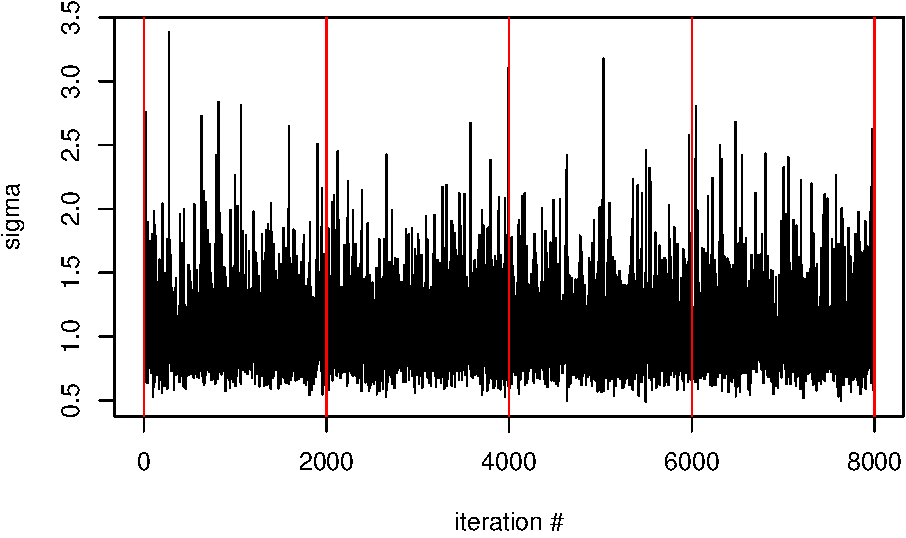
\includegraphics{_main_files/figure-latex/unnamed-chunk-8-1.pdf}

In the next chapter, a more detailed summary of the possibilities of the model specification is given.

\hypertarget{model-specification-details}{%
\chapter{Model specification details}\label{model-specification-details}}

\hypertarget{data_-statements}{%
\section{\texorpdfstring{\texttt{DATA\_*} statements}{DATA\_* statements}}\label{data_-statements}}

The facility for passing data from \texttt{R} to the model is based on the \texttt{DATA\_*} preprocessor macros. Currently there are 6 types of these, corresponding to different types of C++ storage in the model:

\begin{Shaded}
\begin{Highlighting}[]
\NormalTok{DATA\_DOUBLE}\OperatorTok{(\textless{}}\NormalTok{dataname}\OperatorTok{\textgreater{});} \CommentTok{// C++ storage: double }
\NormalTok{DATA\_INT}\OperatorTok{(\textless{}}\NormalTok{dataname}\OperatorTok{\textgreater{});} \CommentTok{// C++ storage: int }
\NormalTok{DATA\_VECTOR}\OperatorTok{(\textless{}}\NormalTok{dataname}\OperatorTok{\textgreater{});} \CommentTok{// C++ storage: Eigen::VectorXd }
\NormalTok{DATA\_IVECTOR}\OperatorTok{(\textless{}}\NormalTok{dataname}\OperatorTok{\textgreater{});} \CommentTok{// C++ storage: Eigen::VectorXi }
\NormalTok{DATA\_MATRIX}\OperatorTok{(\textless{}}\NormalTok{dataname}\OperatorTok{\textgreater{});} \CommentTok{// C++ storage: Eigen::MatrixXd }
\NormalTok{DATA\_IMATRIX}\OperatorTok{(\textless{}}\NormalTok{dataname}\OperatorTok{\textgreater{});} \CommentTok{// C++ storage: Eigen::MatrixXi }
\end{Highlighting}
\end{Shaded}

After putting one or multiple \texttt{DATA\_*} statements at the \textbf{start of the model class}, a object with name \texttt{\textless{}dataname\textgreater{}} and the indicated type will be available throughout the class.

The objects initiated with \texttt{DATA\_*} statements are filled using the \texttt{data} argument of the \texttt{pdmphmc::run} function. E.g. if the model class contains

\begin{Shaded}
\begin{Highlighting}[]
\KeywordTok{struct}\NormalTok{ model}\OperatorTok{\{}
\NormalTok{  DATA\_DOUBLE}\OperatorTok{(}\NormalTok{dd}\OperatorTok{);}
\NormalTok{  DATA\_MATRIX}\OperatorTok{(}\NormalTok{mat}\OperatorTok{);}
  \CommentTok{// rest of model spec here}
\OperatorTok{\};}
\end{Highlighting}
\end{Shaded}

then calls to \texttt{pdmphmc::run} must be done with
something like

\begin{Shaded}
\begin{Highlighting}[]
\CommentTok{\# assuming the model has been built into R{-}variable "model"}
\NormalTok{fit }\OtherTok{\textless{}{-}} \FunctionTok{run}\NormalTok{(model,}\AttributeTok{data=}\FunctionTok{list}\NormalTok{(}\AttributeTok{dd=}\FloatTok{1.23}\NormalTok{,}\AttributeTok{mat=}\FunctionTok{matrix}\NormalTok{(}\FunctionTok{rnorm}\NormalTok{(}\DecValTok{4}\NormalTok{),}\DecValTok{2}\NormalTok{,}\DecValTok{2}\NormalTok{)))}
\end{Highlighting}
\end{Shaded}

The data are read into the C++ program before any sampling etc is done.

\hypertarget{the-preprocess-function}{%
\section{\texorpdfstring{The \texttt{preProcess()} function}{The preProcess() function}}\label{the-preprocess-function}}

The \texttt{preProcess()} is intended for restructuring data, reading data directly from a file etc.

The pre-process function gets called after data are read into C++/is available as objects \texttt{\textless{}dataname\textgreater{}}. E.g. continuing the example above, e.g.

\begin{Shaded}
\begin{Highlighting}[]
\KeywordTok{struct}\NormalTok{ model}\OperatorTok{\{}
\NormalTok{  DATA\_DOUBLE}\OperatorTok{(}\NormalTok{dd}\OperatorTok{);}
\NormalTok{  DATA\_MATRIX}\OperatorTok{(}\NormalTok{mat}\OperatorTok{);}
  \DataTypeTok{double} \VariableTok{ddHalf\_}\OperatorTok{;}
  \DataTypeTok{void}\NormalTok{ preProcess}\OperatorTok{()\{}
    \VariableTok{ddHalf\_} \OperatorTok{=} \FloatTok{0.5}\OperatorTok{*}\NormalTok{dd}\OperatorTok{;}
  \OperatorTok{\}}
  \CommentTok{// rest of model spec here}
\OperatorTok{\};}
\end{Highlighting}
\end{Shaded}

the variable \texttt{ddHalf\_} would contain \texttt{0.5*1.23} at the time of sampling if the same data as above are provided.

\hypertarget{the-operator-function}{%
\section{\texorpdfstring{The \texttt{operator()()} function}{The operator()() function}}\label{the-operator-function}}

The \texttt{operator()()} function is used for specifying (in a broad sense) the target distribution, say \(\pi(\boldsymbol \theta)\).

It should have the signature:

\begin{Shaded}
\begin{Highlighting}[]
\KeywordTok{template} \OperatorTok{\textless{}} \KeywordTok{class}\NormalTok{ varType}\OperatorTok{,} \KeywordTok{class}\NormalTok{ tensorType}\OperatorTok{,} \DataTypeTok{bool}\NormalTok{ storeNames}\OperatorTok{\textgreater{}}
  \DataTypeTok{void} \KeywordTok{operator}\OperatorTok{()(}\NormalTok{amt}\OperatorTok{::}\NormalTok{amtModel}\OperatorTok{\textless{}}\NormalTok{varType}\OperatorTok{,}\NormalTok{tensorType}\OperatorTok{,}\NormalTok{storeNames}\OperatorTok{\textgreater{}} \OperatorTok{\&}\NormalTok{model\_\_}\OperatorTok{)\{}
  \OperatorTok{\}}
\end{Highlighting}
\end{Shaded}

The particular meaning of the templates etc is not important, but the
user should be aware that all parameters, and all quantities depending
on parameters should be of type \texttt{varType}\footnote{So far, \texttt{varType} is either of type \texttt{stan::math::var} or \texttt{amt::amtVar} (see header \texttt{include/amt/amtVar.hpp}).}. \texttt{varType}s could be used more
or less as \texttt{double} types in C++.

Further, the user should be aware of the \texttt{amt::amtModel} object by default named \texttt{model\_\_}\footnote{In principle it could be named something else, but this will break the \texttt{PARAMETER\_*}-macros discussed below. Hence, if the argument to \texttt{operator()} is named something else, the user should provide calls similar to those defined by these macros (see \texttt{include/amt.hpp})}. The \texttt{amt::amtModel} object keeps track of the names and dimensions of the parameters etc, the value of log-target distribution and so on.

\texttt{operator()} typically consist of three parts:

\begin{itemize}
\tightlist
\item
  specifying the sampled quantities \(\boldsymbol \theta\) using \texttt{PARAMETER\_*} macros.
\item
  specifying the shape of the target distribution \(\pi(\boldsymbol \theta)\).
\item
  specifying other quantities of interest for which samples are recorded.
\end{itemize}

In what follows, each of these point are discussed in more detail:

\hypertarget{the-parameter_-macros}{%
\subsection{\texorpdfstring{The \texttt{PARAMETER\_*} macros}{The PARAMETER\_* macros}}\label{the-parameter_-macros}}

The sampled quantities (e.g.~parameters, latent variables and so on) are specified using the \texttt{PARAMETER\_*} macros:

\begin{Shaded}
\begin{Highlighting}[]
\NormalTok{PARAMETER\_SCALAR}\OperatorTok{(\textless{}}\NormalTok{name}\OperatorTok{\textgreater{},...);} \CommentTok{// C++ storage: varType}
\NormalTok{PARAMETER\_VECTOR}\OperatorTok{(\textless{}}\NormalTok{name}\OperatorTok{\textgreater{},}\NormalTok{dim}\OperatorTok{,...);} 
\CommentTok{// C++ storage: Eigen::Matrix\textless{}varType,Eigen::Dynamic,1\textgreater{}  }
\NormalTok{PARAMETER\_MATRIX}\OperatorTok{(}\NormalTok{name}\OperatorTok{,}\NormalTok{dim1}\OperatorTok{,}\NormalTok{dim2}\OperatorTok{,...);} 
\CommentTok{// C++ storage: Eigen::Matrix\textless{}varType,Eigen::Dynamic,Eigen::Dynamic\textgreater{}}
\NormalTok{PARAMETER\_SPD\_MATRIX}\OperatorTok{(}\NormalTok{name}\OperatorTok{,}\NormalTok{dim}\OperatorTok{,...);}
\CommentTok{// C++ storage: amt::SPDmatrix\textless{}varType\textgreater{}}
\end{Highlighting}
\end{Shaded}

All of these macros presume that the argument to the \texttt{operator()}-function is named \texttt{model\_\_}. After a call to e.g.~\texttt{PARAMETER\_VECTOR(\textless{}name\textgreater{},dim,...);}, a vector of \texttt{varType}s of dimension \texttt{dim} and with name \texttt{\textless{}name\textgreater{}} will be available subsequently.

The \texttt{SPDmatrix}class template is further explained in Chapter \ref{amt-SPD-matrix}

An optional argument - the default value - may be passed to each of the
\texttt{PARAMETER\_*} macros. The default value is used when initiating the sampling, and \textbf{it is important that \(\pi(\boldsymbol \theta)\) is defined when \(\boldsymbol \theta\) corresponds to the default values}. If no default values is provided, the default value is implicitly set to \(0\).

(Non-zero) default values could be either \texttt{double} scalars which are repeated to fill non-scalar variables, e.g.

\begin{Shaded}
\begin{Highlighting}[]
\NormalTok{PARAMETER\_VECTOR}\OperatorTok{(}\NormalTok{mu}\OperatorTok{,}\DecValTok{4}\OperatorTok{,}\FloatTok{1.0}\OperatorTok{);}\CommentTok{// mu is intiated at (1.0,1.0,1.0,1.0)}
\end{Highlighting}
\end{Shaded}

Otherwise, the default values may be vectors/matrices of the same dimension(s) as the parameter, e.g.

\begin{Shaded}
\begin{Highlighting}[]
\NormalTok{Eigen}\OperatorTok{::}\NormalTok{Vector muDefault}\OperatorTok{(}\DecValTok{4}\OperatorTok{);}
\NormalTok{muDefault}\OperatorTok{.}\NormalTok{setZero}\OperatorTok{();}
\NormalTok{muDefault}\OperatorTok{(}\DecValTok{3}\OperatorTok{)} \OperatorTok{=} \FloatTok{2.0}\OperatorTok{;}
\NormalTok{PARAMETER\_VECTOR}\OperatorTok{(}\NormalTok{mu}\OperatorTok{,}\NormalTok{muDefault}\OperatorTok{.}\NormalTok{size}\OperatorTok{(),}\NormalTok{muDefault}\OperatorTok{);}
\CommentTok{// mu is intiated at (0.0,0.0,0.0,2.0)}
\end{Highlighting}
\end{Shaded}

One may even pass the dimension and default values of the parameters using the \texttt{DATA\_*}:

\begin{Shaded}
\begin{Highlighting}[]
\KeywordTok{struct}\NormalTok{ model}\OperatorTok{\{}
\NormalTok{  DATA\_VECTOR}\OperatorTok{(}\NormalTok{dvec}\OperatorTok{);}
  \DataTypeTok{void}\NormalTok{ preProcess}\OperatorTok{()\{\}}
  \KeywordTok{template} \OperatorTok{\textless{}} \KeywordTok{class}\NormalTok{ varType}\OperatorTok{,} \KeywordTok{class}\NormalTok{ tensorType}\OperatorTok{,} \DataTypeTok{bool}\NormalTok{ storeNames}\OperatorTok{\textgreater{}}
  \DataTypeTok{void} \KeywordTok{operator}\OperatorTok{()(}\NormalTok{amt}\OperatorTok{::}\NormalTok{amtModel}\OperatorTok{\textless{}}\NormalTok{varType}\OperatorTok{,}\NormalTok{tensorType}\OperatorTok{,}\NormalTok{storeNames}\OperatorTok{\textgreater{}} \OperatorTok{\&}\NormalTok{model\_\_}\OperatorTok{)\{}
\NormalTok{    PARAMETER\_VECTOR}\OperatorTok{(}\NormalTok{d}\OperatorTok{,}\NormalTok{dvec}\OperatorTok{.}\NormalTok{size}\OperatorTok{(),}\NormalTok{dvec}\OperatorTok{);}
    \CommentTok{// d will have the dimension of dvec, and default values=dvec}
    \CommentTok{// rest of model spec here}
  \OperatorTok{\}}
\OperatorTok{\};}
\end{Highlighting}
\end{Shaded}

Note that there are no facilities for specifying that certain elements \(\boldsymbol \theta\) to be restricted to a certain range (e.g.~positive). Hence the user is responsible for ensuring that suitable transformations are made to avoid numerical problems. See e.g.~the log-transformation of the standard deviation in the example in Section \ref{simple-worked-example}

\hypertarget{specifying-the-shape-of-piboldsymbol-theta.}{%
\subsection{\texorpdfstring{Specifying the shape of \(\pi(\boldsymbol \theta)\).}{Specifying the shape of \textbackslash pi(\textbackslash boldsymbol \textbackslash theta).}}\label{specifying-the-shape-of-piboldsymbol-theta.}}

Specifying the shape of the target distribution is done using various overloaded \texttt{+=} operators applied to the \texttt{amt::amtModel} object. It is assumed that \(\log \pi(\boldsymbol \theta)\) may be written as the sum of
several log-densities.

Two sets of such log-densities are available:

\begin{itemize}
\item
  For fixed metric samplers and Riemannian samplers (see Chapter (ref:the-samplers) for details), a library of
  log-densities with names ending with \texttt{\_ld} or \texttt{\_lm} are available under namesspace \texttt{amt}. These are further documented in Chapter \ref{amt-lib}
\item
  For fixed metric samplers only, the complete set of \texttt{stan::math} functions with names ending with \texttt{\_lpdf} or \texttt{\_lpmf} (see \url{https://mc-stan.org/docs/functions-reference/index.html}) are available
\end{itemize}

Below are two examples, both specifying a 4-dimensional standard normal target distribution:

\begin{Shaded}
\begin{Highlighting}[]
\CommentTok{//...}
  \KeywordTok{template} \OperatorTok{\textless{}} \KeywordTok{class}\NormalTok{ varType}\OperatorTok{,} \KeywordTok{class}\NormalTok{ tensorType}\OperatorTok{,} \DataTypeTok{bool}\NormalTok{ storeNames}\OperatorTok{\textgreater{}}
  \DataTypeTok{void} \KeywordTok{operator}\OperatorTok{()(}\NormalTok{amt}\OperatorTok{::}\NormalTok{amtModel}\OperatorTok{\textless{}}\NormalTok{varType}\OperatorTok{,}\NormalTok{tensorType}\OperatorTok{,}\NormalTok{storeNames}\OperatorTok{\textgreater{}} \OperatorTok{\&}\NormalTok{model\_\_}\OperatorTok{)\{}
\NormalTok{    PARAMETER\_VECTOR}\OperatorTok{(}\NormalTok{x}\OperatorTok{,}\DecValTok{4}\OperatorTok{);}
\NormalTok{    model\_\_ }\OperatorTok{+=}\NormalTok{ normal\_ld}\OperatorTok{(}\NormalTok{x}\OperatorTok{,}\FloatTok{0.0}\OperatorTok{,}\FloatTok{1.0}\OperatorTok{);} \CommentTok{// amt version}
  \OperatorTok{\}}
\CommentTok{//...}
\end{Highlighting}
\end{Shaded}

\begin{Shaded}
\begin{Highlighting}[]
\CommentTok{//...}
  \KeywordTok{template} \OperatorTok{\textless{}} \KeywordTok{class}\NormalTok{ varType}\OperatorTok{,} \KeywordTok{class}\NormalTok{ tensorType}\OperatorTok{,} \DataTypeTok{bool}\NormalTok{ storeNames}\OperatorTok{\textgreater{}}
  \DataTypeTok{void} \KeywordTok{operator}\OperatorTok{()(}\NormalTok{amt}\OperatorTok{::}\NormalTok{amtModel}\OperatorTok{\textless{}}\NormalTok{varType}\OperatorTok{,}\NormalTok{tensorType}\OperatorTok{,}\NormalTok{storeNames}\OperatorTok{\textgreater{}} \OperatorTok{\&}\NormalTok{model\_\_}\OperatorTok{)\{}
\NormalTok{    PARAMETER\_VECTOR}\OperatorTok{(}\NormalTok{x}\OperatorTok{,}\DecValTok{4}\OperatorTok{);}
\NormalTok{    model\_\_ }\OperatorTok{+=}\NormalTok{ stan}\OperatorTok{::}\NormalTok{math}\OperatorTok{::}\NormalTok{normal\_lpdf}\OperatorTok{(}\NormalTok{x}\OperatorTok{,}\FloatTok{0.0}\OperatorTok{,}\FloatTok{1.0}\OperatorTok{);} \CommentTok{// stan::math version}
  \OperatorTok{\}}
\CommentTok{//...}
\end{Highlighting}
\end{Shaded}

Further, more elaborate examples of model specifications are provided in Chapter \ref{worked-examples}.

\hypertarget{generated-quantities}{%
\subsection{Generated quantities}\label{generated-quantities}}

Generated quantities are used in two ways:

\begin{itemize}
\item
  It is often the case that one is interested in the posterior distribution of some auxiliary quantities which depend on the parameter \(\boldsymbol \theta\).
\item
  The \texttt{pdmphmc} package has the capability to compute ``time-integrated'' samples (see e.g. \citet{kleppe_CTHMC}, Equation 7 and Figure 3), which in certain cases may be much more efficient for estimating certain moments. Time integrated samples are computed for all generated quantities (and not the parameters, so if you want time-integrated samples of the parameters, pass them as generated quantities).
\end{itemize}

To record such quantities, the \texttt{generated()} function (member of \texttt{amt::amtModel}) is used. There are several overloads of \texttt{generated()} allowing several types (scalars, vectors, matrices etc.) to be passed.

The \texttt{generated()} functions have signatures similar to
\texttt{inline\ void\ generated(const\ \textless{}SOME\ TYPE\textgreater{}\&\ value,const\ std::string\&\ name)}, where \texttt{\textless{}SOME\ TYPE\textgreater{}} is a C++ type/template, such as e.g.~\texttt{double}, \texttt{Eigen::VectorXd} or \texttt{varType}. \texttt{name} is the name used for the generated quantity in the output.

Below is a complete example of the usage. First, the content of file \texttt{generated\_model.cpp}:

\begin{Shaded}
\begin{Highlighting}[]
\KeywordTok{using} \KeywordTok{namespace}\NormalTok{ amt}\OperatorTok{;}

\DataTypeTok{double}\NormalTok{ quadNorm}\OperatorTok{(}\AttributeTok{const}\NormalTok{ Eigen}\OperatorTok{::}\NormalTok{VectorXd}\OperatorTok{\&}\NormalTok{ x}\OperatorTok{)\{}
  \ControlFlowTok{return}\OperatorTok{(}\NormalTok{x}\OperatorTok{.}\NormalTok{dot}\OperatorTok{(}\NormalTok{x}\OperatorTok{));}
\OperatorTok{\}}

\KeywordTok{struct}\NormalTok{ model}\OperatorTok{\{}
  \DataTypeTok{void}\NormalTok{ preProcess}\OperatorTok{()\{\}} \CommentTok{// not used in this example }
  \KeywordTok{template} \OperatorTok{\textless{}} \KeywordTok{class}\NormalTok{ varType}\OperatorTok{,} \KeywordTok{class}\NormalTok{ tensorType}\OperatorTok{,} \DataTypeTok{bool}\NormalTok{ storeNames}\OperatorTok{\textgreater{}}
  \DataTypeTok{void} \KeywordTok{operator}\OperatorTok{()(}\NormalTok{amt}\OperatorTok{::}\NormalTok{amtModel}\OperatorTok{\textless{}}\NormalTok{varType}\OperatorTok{,}\NormalTok{tensorType}\OperatorTok{,}\NormalTok{storeNames}\OperatorTok{\textgreater{}} \OperatorTok{\&}\NormalTok{model\_\_}\OperatorTok{)\{}
    
\NormalTok{    PARAMETER\_VECTOR}\OperatorTok{(}\NormalTok{x}\OperatorTok{,}\DecValTok{4}\OperatorTok{);} \CommentTok{// parameter (sampled quantity)}
\NormalTok{    model\_\_}\OperatorTok{+=}\NormalTok{normal\_ld}\OperatorTok{(}\NormalTok{x}\OperatorTok{,}\FloatTok{0.0}\OperatorTok{,}\FloatTok{1.0}\OperatorTok{);} \CommentTok{// add standard normal log{-}density}
    
    
    \CommentTok{// make the whole parameter a generated}
\NormalTok{    model\_\_}\OperatorTok{.}\NormalTok{generated}\OperatorTok{(}\NormalTok{asDouble}\OperatorTok{(}\NormalTok{x}\OperatorTok{),}\StringTok{"x\_gen"}\OperatorTok{);} 
    \CommentTok{// different transformations of x to be recored:}
\NormalTok{    model\_\_}\OperatorTok{.}\NormalTok{generated}\OperatorTok{(}\BuiltInTok{std::}\NormalTok{pow}\OperatorTok{(}\NormalTok{asDouble}\OperatorTok{(}\NormalTok{x}\OperatorTok{(}\DecValTok{0}\OperatorTok{)),}\DecValTok{3}\OperatorTok{),}\StringTok{"x1\_cube"}\OperatorTok{);}
\NormalTok{    model\_\_}\OperatorTok{.}\NormalTok{generated}\OperatorTok{(}\NormalTok{exp}\OperatorTok{(}\NormalTok{asDouble}\OperatorTok{(}\NormalTok{x}\OperatorTok{(}\DecValTok{1}\OperatorTok{))),}\StringTok{"x2\_exp"}\OperatorTok{);}
    
    \DataTypeTok{double}\NormalTok{ qn }\OperatorTok{=}\NormalTok{ quadNorm}\OperatorTok{(}\NormalTok{asDouble}\OperatorTok{(}\NormalTok{x}\OperatorTok{));}
\NormalTok{    model\_\_}\OperatorTok{.}\NormalTok{generated}\OperatorTok{(}\NormalTok{qn}\OperatorTok{,}\StringTok{"quadraticNorm"}\OperatorTok{);}
    
  \OperatorTok{\}} 
\OperatorTok{\};} \CommentTok{// end of struct}
\end{Highlighting}
\end{Shaded}

Note that it is good practice to provide \texttt{double} values as the first argument to \texttt{generated()}. The double value of AD types \texttt{varType} obtains using the \texttt{asDouble()} function.

Then build and run the model:

\begin{Shaded}
\begin{Highlighting}[]
\NormalTok{model }\OtherTok{\textless{}{-}}\NormalTok{ pdmphmc}\SpecialCharTok{::}\FunctionTok{build}\NormalTok{(}\StringTok{"generated\_model.cpp"}\NormalTok{)}
\end{Highlighting}
\end{Shaded}

\begin{verbatim}
## model name : model
\end{verbatim}

\begin{verbatim}
## process type : HMCProcess
\end{verbatim}

\begin{verbatim}
## metric tensor type : metricTensorDummy
\end{verbatim}

\begin{verbatim}
## compilation exited successfully
\end{verbatim}

\begin{Shaded}
\begin{Highlighting}[]
\NormalTok{fit }\OtherTok{\textless{}{-}}\NormalTok{ pdmphmc}\SpecialCharTok{::}\FunctionTok{run}\NormalTok{(model)}
\NormalTok{fit}
\end{Highlighting}
\end{Shaded}

\begin{verbatim}
## run output for model: model
\end{verbatim}

\begin{verbatim}
## # of chains : 4
\end{verbatim}

\begin{verbatim}
## Summary based on discrete samples:
\end{verbatim}

\begin{verbatim}
##                 mean se_mean    sd n_eff  Rhat
## x[1]          -0.017   0.017 0.973  3391 1.003
## x[2]           0.007   0.017 1.037  3546 1.004
## x[3]           0.006   0.017 1.024  3736 1.000
## x[4]           0.006   0.017 0.977  3329 1.002
## x_gen[1]      -0.017   0.017 0.973  3391 1.003
## x_gen[2]       0.007   0.017 1.037  3546 1.004
## x_gen[3]       0.006   0.017 1.024  3736 1.000
## x_gen[4]       0.006   0.017 0.977  3329 1.002
## x1_cube       -0.032   0.058 3.627  3849 1.003
## x2_exp         1.719   0.039 2.305  3440 1.003
## quadraticNorm  4.026   0.068 2.846  1720 1.001
\end{verbatim}

\begin{verbatim}
## summary based on integrated samples:
\end{verbatim}

\begin{verbatim}
##               estimate se_estimate n_eff  Rhat
## x_gen[1]         0.005       0.005  5963 1.005
## x_gen[2]         0.003       0.005  5811 1.002
## x_gen[3]         0.004       0.005  6267 1.000
## x_gen[4]        -0.003       0.005  5968 0.999
## x1_cube          0.008       0.018  6574 1.006
## x2_exp           1.718       0.038   989 1.003
## quadraticNorm    4.043       0.067   838 1.003
\end{verbatim}

\begin{verbatim}
## NOTE: integrated samples do NOT reflect the complete target distibution, only indicated moments with respect to the target distribution
\end{verbatim}

It is seen that discrete time samples (which reflect target distribution) are recorded (by default) for the parameters (in this case \texttt{x{[}1{]}},\ldots,\texttt{x{[}4{]}}) and the generated quantities (here \texttt{x\_gen{[}1{]}},\ldots,\texttt{x\_gen{[}4{]}},\texttt{x1\_cube},\texttt{x2\_exp},\texttt{quadraticNorm}).

Integrated samples for calculating moments with respect to the target distribution are recorded for the generated quantities only.

Some minor comments related to performance are in order here:

\begin{itemize}
\item
  As seen in the example above, \texttt{double} values (or vectors or matrices thereof) should ideally be passed to the \texttt{generated()} functions. This is in order of avoiding unnecessary AD computations. In particular, if the generated function is a complicated function of the parameters (for which function \texttt{quadNorm()} may serve as a placeholder), the computations leading up to the generated quantity should be done in double-variables.
\item
  In models where \(\boldsymbol \theta\) is high-dimensional and parts of \(\boldsymbol \theta\) are of less interest, the default behavior of storing samples of all of \(\boldsymbol \theta\) may be overridden by using the \texttt{store.pars} argument in \texttt{pdmphmc::run()}. Reducing the number of stored quantities leads to both memory savings and savings in terms of computing time.
\end{itemize}

\hypertarget{amt-lib}{%
\chapter{\texorpdfstring{The \texttt{amt}-library}{The amt-library}}\label{amt-lib}}

This section gives an overview of the different probability density/mass functions, in addition to some utility functions available in the \texttt{amt}-library. The library provides an automatic
implementation of the methodology of \citet{kleppe_amt} for automatically computing a ``metric tensors'' suitable Riemannian sampling algorithms for arbitrary models.

The design of the library allows the user to use the same model specification for both Riemannian and regular fixed metric sampling (see Chapter \ref{the-samplers}).

The methodology of \citet{kleppe_amt} generally requires that all probability densities involved in the model where the argument depends on \(\boldsymbol \theta\) (generally the conditional densities of priors and latent variables) to have continuous first order derivatives. To achieve such continuity, many of the below distributions are known probability distributions that have been transformed to have support on the whole real line in such a way that the resulting probability distribution is sufficiently smooth. These transformations are also desirable from a numerical point of view.

As a basic example of such transformations involves the \(ExpGamma\)-distribution (see below for proper definition):

\begin{Shaded}
\begin{Highlighting}[]
\CommentTok{// inside operator()()}
\NormalTok{PARAMETER\_SCALAR}\OperatorTok{(}\NormalTok{logSigma}\OperatorTok{,}\FloatTok{0.0}\OperatorTok{);}
\NormalTok{model\_\_}\OperatorTok{+=}\NormalTok{expGamma\_ld}\OperatorTok{(}\NormalTok{logSigma}\OperatorTok{,}\FloatTok{1.0}\OperatorTok{,}\FloatTok{1.0}\OperatorTok{);}
\NormalTok{varType sigma}\OperatorTok{=}\NormalTok{exp}\OperatorTok{(}\NormalTok{logSigma}\OperatorTok{);} 
\NormalTok{model\_\_}\OperatorTok{.}\NormalTok{generated}\OperatorTok{(}\NormalTok{asDouble}\OperatorTok{(}\NormalTok{sigma}\OperatorTok{),}\StringTok{"sigma"}\OperatorTok{);}
\end{Highlighting}
\end{Shaded}

In the above example, \texttt{sigma} will be exponentially distributed with mean 1 (until further conditioning is done) and will be recorded as a generated quantity.

\hypertarget{amt-SPD-matrix}{%
\section{Utilities for symmetric positive definite matrices}\label{amt-SPD-matrix}}

The \texttt{amt}-package provides a set of utilities for representing symmetric positive definite (SPD) matrices. Internally, this class template \texttt{SPDmatrix} represents a \(d \times d\) SPD matrix as an ``internal'' vector of \(d(d+1)/2\) \texttt{varTypes}.

\texttt{SPDmatrix} objects may be used as e.g.~covariance- or precision matrices in multivariate normal distributions, and it also possible to assign e.g.~Wishart distributions on such objects (though in practice, such assignments are really distributions on the internal vector, consistent with the matrix-valued distribution).

The easiest way to construct a \texttt{SPDmatrix} is via the \texttt{PARAMETER\_SPD\_MATRIX(name,dim,...)} macro. Typical usage involves something like:

\begin{Shaded}
\begin{Highlighting}[]
\CommentTok{// inside operator()() : }
\NormalTok{PARAMETER\_SPD\_MATRIX}\OperatorTok{(}\NormalTok{P}\OperatorTok{,}\DecValTok{3}\OperatorTok{);} 
\CommentTok{// Note: PARAMETER\_SPD\_MATRIX(P,3) really makes a parameter vector  }
\CommentTok{// named P\_internal, and subsequently constructs SPDmatrix\textless{}varType\textgreater{} P}
\NormalTok{Eigen}\OperatorTok{::}\NormalTok{VectorXd scaleDiag}\OperatorTok{;}\NormalTok{ scaleDiag}\OperatorTok{.}\NormalTok{setConstant}\OperatorTok{(}\DecValTok{3}\OperatorTok{,}\FloatTok{4.0}\OperatorTok{);}
\NormalTok{model\_\_ }\OperatorTok{+=}\NormalTok{ wishartDiagScale\_ld}\OperatorTok{(}\NormalTok{P}\OperatorTok{,}\NormalTok{scaleDiag}\OperatorTok{,}\FloatTok{10.0}\OperatorTok{);} 
\CommentTok{// P has a Wishart(4*I,10.0) distribution a priori }
\NormalTok{model\_\_}\OperatorTok{.}\NormalTok{generated}\OperatorTok{(}\NormalTok{P}\OperatorTok{,}\StringTok{"P"}\OperatorTok{);} \CommentTok{// full matrix stored}
\NormalTok{model\_\_}\OperatorTok{.}\NormalTok{generated}\OperatorTok{(}\NormalTok{P}\OperatorTok{.}\NormalTok{coeff}\OperatorTok{(}\DecValTok{0}\OperatorTok{,}\DecValTok{2}\OperatorTok{),}\StringTok{"P13"}\OperatorTok{);} \CommentTok{// single element stored}
\end{Highlighting}
\end{Shaded}

A complete class where the above code block is the body of the \texttt{operator()()}-method is stored in the file \texttt{wishart\_example.cpp}, which is built an run via:

\begin{Shaded}
\begin{Highlighting}[]
\NormalTok{mdl }\OtherTok{\textless{}{-}}\NormalTok{ pdmphmc}\SpecialCharTok{::}\FunctionTok{build}\NormalTok{(}\StringTok{"wishart\_example.cpp"}\NormalTok{)}
\end{Highlighting}
\end{Shaded}

\begin{verbatim}
## model name : model
\end{verbatim}

\begin{verbatim}
## process type : HMCProcess
\end{verbatim}

\begin{verbatim}
## metric tensor type : metricTensorDummy
\end{verbatim}

\begin{verbatim}
## compilation exited successfully
\end{verbatim}

\begin{Shaded}
\begin{Highlighting}[]
\NormalTok{fit }\OtherTok{\textless{}{-}}\NormalTok{ pdmphmc}\SpecialCharTok{::}\FunctionTok{run}\NormalTok{(mdl)}
\NormalTok{fit}
\end{Highlighting}
\end{Shaded}

\begin{verbatim}
## run output for model: model
\end{verbatim}

\begin{verbatim}
## # of chains : 4
\end{verbatim}

\begin{verbatim}
## Summary based on discrete samples:
\end{verbatim}

\begin{verbatim}
##                 mean se_mean     sd n_eff  Rhat
## P_internal[1]  3.570   0.010  0.491  2369 1.002
## P_internal[2]  3.468   0.010  0.492  2455 1.004
## P_internal[3]  3.330   0.010  0.542  3228 1.001
## P_internal[4]  0.000   0.007  0.366  3128 1.002
## P_internal[5] -0.008   0.007  0.362  2862 1.001
## P_internal[6]  0.008   0.007  0.377  2577 1.002
## P[1,1]        39.708   0.370 18.407  2467 1.002
## P[2,1]         0.134   0.229 12.988  3225 1.002
## P[3,1]        -0.025   0.241 12.947  2874 1.000
## P[2,2]        40.107   0.347 17.647  2581 1.003
## P[3,2]         0.284   0.248 12.982  2726 1.003
## P[3,3]        40.197   0.305 18.000  3479 1.002
## P13           -0.025   0.241 12.947  2874 1.000
\end{verbatim}

\begin{verbatim}
## summary based on integrated samples:
\end{verbatim}

\begin{verbatim}
##        estimate se_estimate n_eff  Rhat
## P[1,1]   39.707       0.184  1838 1.005
## P[2,1]    0.028       0.056  7138 1.034
## P[3,1]    0.053       0.053  6941 1.029
## P[2,2]   40.200       0.182  1768 1.001
## P[3,2]    0.144       0.101  2184 1.002
## P[3,3]   40.235       0.163  2335 1.001
## P13       0.053       0.053  6941 1.029
\end{verbatim}

\begin{verbatim}
## NOTE: integrated samples do NOT reflect the complete target distibution, only indicated moments with respect to the target distribution
\end{verbatim}

Notice that by default, the ``internal'' parameter vector \texttt{P\_internal} is stored\footnote{This may be avoided by using the \texttt{store.pars}-option in \texttt{pdmphmc::run()}.} in addition to the generated quantities. Note, in this case, we would expect \(E(\mathbf P)=40 \mathbf I\).

\hypertarget{univariate-continuous-distributions}{%
\section{Univariate continuous distributions}\label{univariate-continuous-distributions}}

\hypertarget{expgamma_ldargshapescale}{%
\subsection{\texorpdfstring{\texttt{expGamma\_ld(arg,shape,scale)}}{expGamma\_ld(arg,shape,scale)}}\label{expgamma_ldargshapescale}}

The distribution obtained by applying the (natural) logarithm to a gamma-distributed random variable with shape parameter \(\alpha=\)\texttt{shape} and scale parameter \(\beta=\)\texttt{scale}. Argument of resulting PDF \(x=\)\texttt{arg}. Log-density:
\[
\log p(x|\alpha,\beta) = -a\log(b) - \log(\Gamma(a)) + ax - \exp(x)/b.
\]

\hypertarget{invlogitbeta_ldxab}{%
\subsection{\texorpdfstring{\texttt{invLogitBeta\_ld(x,a,b)}}{invLogitBeta\_ld(x,a,b)}}\label{invlogitbeta_ldxab}}

The distribution obtained by applying the logit-function to a Beta distributed random variable with shape parameters \texttt{a} and \texttt{b}. Argument of resulting PDF: \(x=\)\texttt{x}. Log-density:
\[
\log p(x|a,b) = \log(\Gamma(a+b)) - \log(\Gamma(a)\Gamma(b)) + a\log\left(\frac{\exp(x)}{1+\exp(x)}\right) - b\log(1+\exp(x)).
\]

\hypertarget{invlogituniform_ldx}{%
\subsection{\texorpdfstring{\texttt{invLogitUniform\_ld(x)}}{invLogitUniform\_ld(x)}}\label{invlogituniform_ldx}}

The distribution obtained by applying the logit-function to a uniform(0,1); same as the standard logistic distribution. Argument of resulting PDF: \(x=\)\texttt{x}. Log-density:
\[
\log p(x) = x - 2\log(1+\exp(x))
\]

\hypertarget{normal_ldargmeansd}{%
\subsection{\texorpdfstring{\texttt{normal\_ld(arg,mean,sd)}}{normal\_ld(arg,mean,sd)}}\label{normal_ldargmeansd}}

Normal/Gaussian distribution with mean=\texttt{mean} and standard deviation=\texttt{sd}. Argument of PDF: \(x=\)\texttt{arg}.

\hypertarget{univariate-discrete-distributions}{%
\section{Univariate discrete distributions}\label{univariate-discrete-distributions}}

\hypertarget{bernoulli_logit_lmyalpha}{%
\subsection{\texorpdfstring{\texttt{bernoulli\_logit\_lm(y,alpha)}}{bernoulli\_logit\_lm(y,alpha)}}\label{bernoulli_logit_lmyalpha}}

Bernoulli-distribution with \(P(y=1)=\exp(\alpha)/(1+\exp(\alpha))\). Argument \(y\) is of integer type.

\hypertarget{poisson_log_lmyeta}{%
\subsection{\texorpdfstring{\texttt{poisson\_log\_lm(y,eta)}}{poisson\_log\_lm(y,eta)}}\label{poisson_log_lmyeta}}

Poisson distribution with mean equal to \(\exp(\eta)\). Argument \(y\) is of integer type.

\hypertarget{zipoisson_log_lmyetag}{%
\subsection{\texorpdfstring{\texttt{ziPoisson\_log\_lm(y,eta,g)}}{ziPoisson\_log\_lm(y,eta,g)}}\label{zipoisson_log_lmyetag}}

Zero-inflated Poisson distribution. A mixture of point-mass at \(y=0\) (with weight \(p\)) and a regular Poisson distribution with mean \(\exp(\eta)\) (with weight \(1-p\)). \(g=\text{logit}(p)\).

\hypertarget{distributions-on-unbounded-vectors}{%
\section{Distributions on unbounded vectors}\label{distributions-on-unbounded-vectors}}

\hypertarget{multi_normal_prec_ldargmuprec}{%
\subsection{\texorpdfstring{\texttt{multi\_normal\_prec\_ld(arg,mu,Prec)}}{multi\_normal\_prec\_ld(arg,mu,Prec)}}\label{multi_normal_prec_ldargmuprec}}

Multivariate normal distribution where the \textbf{precision} matrix \texttt{Prec} is a \texttt{SPDmatrix} (see Section \ref{amt-SPD-matrix}). Both the argument \texttt{arg} and \texttt{mean} are vectors with dimension equal to \texttt{Prec.dim()}.

\hypertarget{iid_multi_normal_prec_ldargmuprec}{%
\subsection{\texorpdfstring{\texttt{iid\_multi\_normal\_prec\_ld(arg,mu,Prec)}}{iid\_multi\_normal\_prec\_ld(arg,mu,Prec)}}\label{iid_multi_normal_prec_ldargmuprec}}

Same as above, but \texttt{arg} is now a matrix, where the columns are iid realizations from \(N(\mu,P^{-1})\), where \(P=\)\texttt{Prec}.

\hypertarget{multi_normal_ldargmusigma}{%
\subsection{\texorpdfstring{\texttt{multi\_normal\_ld(arg,mu,Sigma)}}{multi\_normal\_ld(arg,mu,Sigma)}}\label{multi_normal_ldargmusigma}}

Multivariate normal distribution where the \textbf{covariance} matrix \texttt{Sigma} is a \texttt{SPDmatrix} (see Section \ref{amt-SPD-matrix}). Both the argument \texttt{arg} and \texttt{mean} are vectors with dimension equal to \texttt{Sigma.dim()}.

To do: iid-variant of this.

\hypertarget{normalar1_ldargmuphisigma}{%
\subsection{\texorpdfstring{\texttt{normalAR1\_ld(arg,mu,phi,sigma)}}{normalAR1\_ld(arg,mu,phi,sigma)}}\label{normalar1_ldargmuphisigma}}

Stationary Gaussian first order autoregressive process

\[
x_1 \sim N\left (\mu,\frac{\sigma^2}{1-\phi^2} \right), x_{t} = \mu + \phi ( x_{t-1}-\mu) + N(0,\sigma^2),t=2,\dots,T\;
\]
for scalar parameters \(\mu\), \(-1<\phi<1\) and \(\sigma>0\). \(\mathbf x=\)\texttt{arg} is a \(T\)-dimensional vector.

\hypertarget{normalrw1_ldxsigma}{%
\subsection{\texorpdfstring{\texttt{normalRW1\_ld(x,sigma)}}{normalRW1\_ld(x,sigma)}}\label{normalrw1_ldxsigma}}

First order (intrinsic) Gaussian random walk model:
\[
x_t \sim N(x_{t-1},\sigma^2),\; t=2,\dots,T,
\]
for \(\sigma>0\). \(\mathbf x=\)\texttt{x} is a \(T\)-dimensional vector. Note that this model specifies a degenerate probability distribution, and \(\mathbf x\) cannot be sampled without further conditioning.

\hypertarget{distributions-on-symmetric-positive-definite-matrices}{%
\section{Distributions on symmetric positive definite matrices}\label{distributions-on-symmetric-positive-definite-matrices}}

The notation for the Wishart distribution is \(\mathcal W(\mathbf M,\nu)\) where \(\mathbf M\) is the scale matrix and \(\nu\) is the degrees of freedom parameter. Consequently, if \(\mathbf P \sim \mathcal W(\mathbf M,\nu)\), then \(E(\mathbf P)=\nu \mathbf M\).

\hypertarget{wishartdiagscale_ldargscalediagdf}{%
\subsection{\texorpdfstring{\texttt{wishartDiagScale\_ld(arg,scaleDiag,df)}}{wishartDiagScale\_ld(arg,scaleDiag,df)}}\label{wishartdiagscale_ldargscalediagdf}}

The Wishart distribution \(\mathbf P \sim \mathcal W(\mathbf M,\nu)\) where \(\mathbf P=\)\texttt{arg} is a \texttt{SPDmatrix}, vector \(\text{diag}(\mathbf M)\)=\texttt{scaleDiag} and scalar \(\nu=\)\texttt{df}.

\hypertarget{wishartrw1_ldargmeannu}{%
\subsection{\texorpdfstring{\texttt{wishartRW1\_ld(arg,mean,nu)}}{wishartRW1\_ld(arg,mean,nu)}}\label{wishartrw1_ldargmeannu}}

The Wishart distribution \(\mathbf P \sim \mathcal W(\nu^{-1}\mathbf Q,\nu)\). \(\mathbf P=\)\texttt{arg} is a \texttt{SPDmatrix}, \(E(\mathbf P)=\mathbf Q=\)\texttt{mean} is a \texttt{SPDmatrix} and scalar \(\nu=\)\texttt{nu}.

\hypertarget{the-samplers}{%
\chapter{The sampling algorithms}\label{the-samplers}}

As the name of the package indicates, the samplers in employed in this package are based on piecewise deterministic Markov processes (see e.g. \citet{fearnhead2018}) with Hamiltonian dynamic between events (see \citet{kleppe_CTHMC}).

Two distinct such samplers are so far implemented: fixed mass (section \ref{fixed-mass-sampler}) and Riemannian manifold (Section \ref{Riemann-manifold}). The Hamiltonians, which are fully specifies the between event dynamics are provided below.

The same set of numerical differential equation solvers (Section \ref{ODE-solvers}) are used for both solvers. Finally, methods for adapting the scaling of the differential equations (Section \ref{scaling-adaptation}) and the different available event intensities (Section \ref{event-intensity}) are described below.

The sampling algorithm to be used are chosen prior to the compilation \texttt{pdmphmc::build()}. By default, a fixed mass sampler is used.

Whether to use the RM sampler or fixed metric sampler is inherently problem-specific. As a rule of thumb, if your target distribution involves complicated non-linear dependencies, or the scale of some subset of \(\boldsymbol \theta\) depends strongly on some other subset of \(\boldsymbol \theta\), the RM sampler is often a good choice. However, the differential equations associated with the RM sampler are more expensive to compute than for the fixed metric sampler. Hence, if it is possible to rewrite your model so that the fixed metric sampler gives good results (see e.g. \citet{doi:10.1080/10618600.2019.1584901} or \citet{1812.07929}), this approach is often a good choice.

\hypertarget{fixed-mass-sampler}{%
\section{Fixed mass sampler}\label{fixed-mass-sampler}}

Suppose the target density is given by \(\pi (\boldsymbol \theta)\) and that the model specification admits the evaluation \(\bar \pi(\boldsymbol \theta) \propto \pi (\boldsymbol \theta)\). The Hamiltonian \(\mathcal H(\mathbf q,\mathbf p)\) used to define the deterministic dynamics for the fixed mass sampler is
\[
\mathcal H(\mathbf q,\mathbf p) = -\log \pi(\mathbf m + \mathbf S \mathbf q) + \frac{1}{2} \mathbf p^T \mathbf p.
\]
Here \(\mathbf p\) is the (fictitious) momentum variable introduced to construct a dynamical system with Boltzmann-Gibbs distribution \(\pi(\mathbf q, \mathbf p) \propto \exp(-\mathcal H(\mathbf q,\mathbf p))\).

Samples are subsequently recorded for \(\boldsymbol \theta=\mathbf m + \mathbf S \mathbf q\) which will be distributed according to \(\pi(\boldsymbol \theta)\). Here vector \(\mathbf m\) and diagonal positive definite matrix \(\mathbf S\) are adapted during the warmup process (see Chapter \ref{scaling-adaptation})

The vector \(\mathbf m\) should reflect the mean of the target distribution, and the diagonal elements of \(\mathbf S\) should reflect the scale properties of \(\boldsymbol \theta\) under the target distribution.

The reasoning behind introducing the re-parameterization \(\mathbf q \leftrightarrow \boldsymbol \theta\) (rather than to account for different scales by introducing a non-identity mass matrix in the kinetic energy term of \(\mathcal H(\mathbf q,\mathbf p)\))
is based on the desire for obtaining well-scaled Hamilton's equations
\[
\dot{ \mathbf q}(t) = \mathbf p(t)
\]
\[
\dot{\mathbf p}(t) = \mathbf S \mathbf g(\mathbf m+\mathbf S \mathbf q(t)), \; \mathbf g(\boldsymbol \theta) = \nabla_{\boldsymbol \theta}\log \pi (\boldsymbol \theta)
\]
suitable for numerical integration. I.e. for suitably chosen \(\mathbf S\) the force term in both equations should have order \(1\) (as \(Var(\mathbf p)=\mathbf I\) under the Boltzmann-Gibbs distribution).

The sampler is chosen explicitly by selecting \texttt{process.type\ =\ "HMCProcess"} in the call to \texttt{pdmphmc::build()}, but as mentioned is already the default option.

\hypertarget{Riemann-manifold}{%
\section{Riemann manifold sampler}\label{Riemann-manifold}}

The Riemann manifold (RM) sampler is based on the availability of a ``metric tensor'' \(\mathbf G(\boldsymbol \theta)\). Namely for each \(\boldsymbol \theta\), then \(\mathbf G(\boldsymbol \theta)\) is a symmetric positive definite matrix that may be interpreted as the ``local precision matrix'' of the target distribution.

The \texttt{amt}-library provides an automatic methodology for computing metric tensors from a given model specification (see \citet{kleppe_amt} for details), and by default this methodology is used if the RM sampler is selected via \texttt{process.type\ =\ "RMHMCProcess"} in the call to \texttt{pdmphmc::build()}.

The Hamiltonian for the RM sampler is given by
\[
\mathcal H(\mathbf q,\mathbf p) = -\log \bar \pi(\mathbf m + \mathbf S \mathbf q) + \frac{1}{2}\log(|\bar{\mathbf G}(\mathbf q)|) + \frac{1}{2}\mathbf p^T[\bar{\mathbf G}(\mathbf q)]^{-1}\mathbf p
\]
where
\[
\bar{\mathbf G}(\mathbf q) = \mathbf S^T \mathbf G(\mathbf m + \mathbf S \mathbf q) \mathbf S.
\]

It is seen that the interpretation of \(\mathbf m\) and \(\mathbf S\) are the same also for the RM sampler, i.e.~\(\mathbf m\) should reflect the center/mean of the distribution, and \(\mathbf S\) should reflect the scale of each element in \(\boldsymbol \theta\).

\hypertarget{metric-tensor-storage}{%
\subsection{Metric tensor storage}\label{metric-tensor-storage}}

Two storage schemes for the metric tensor are available

\begin{itemize}
\item
  sparse storage using on the \texttt{ldl} Cholesky factorization (\citet{davis_ldl})
\item
  dense storage using the Cholesky factorization of the Stan math library.
\end{itemize}

One should use the sparse storage scheme if the metric tensor is very sparse, which is often the case for hierarchical models.
The metric tensor scheme is chosen during the \texttt{pdmphmc::build()}-process by selecting \texttt{metric.tensor.type\ =\ c("Sparse",\ "Dense")}.

Note that for the sparse storage scheme, the ordering of the parameters may play a role for the performance of the Cholesky factorization (see \citet{davis_sparse}). The ordering of the parameters are determined by the ordering of the \texttt{PARAMETER\_*} statements in the model specification.

\hypertarget{advanced}{%
\subsection{Advanced}\label{advanced}}

It is also possible to specify ones own metric tensor. One turns off the default \texttt{amt}-library metric tensor by choosing the option \texttt{amt=FALSE} in the call to \texttt{pdmphmc::build()}. This process will be documented in more detail soon.

\hypertarget{ODE-solvers}{%
\section{ODE solvers}\label{ODE-solvers}}

So far, only the order 5 (4) pair of \citet{DORMAND198019} with dense output is used for integrating the differential equations. A PI controller is used for adaptive time step sizes.

\hypertarget{scaling-adaptation}{%
\section{Scaling adaptation}\label{scaling-adaptation}}

So far, only square-roots of estimates of the diagonal elements of \(Var(\boldsymbol \theta)\) are available as the diagonal elements of \(\mathbf S\). See \citet{kleppe_CTHMC} for details

\hypertarget{event-intensity}{%
\section{Event intensity}\label{event-intensity}}

So far, only constant event intensities are available. See \citet{kleppe_CTHMC} for details on on the adaptive choice of this constant event intensity.

\hypertarget{worked-examples}{%
\chapter{Worked examples}\label{worked-examples}}

More to come here.

  \bibliography{book.bib,packages.bib}

\end{document}
